%!TEX root = main.tex

\section{Revisão da Literatura}

A revisão de literatura consiste na apresentação, síntese e avaliação crítica da dita literatura, de modo a sustentar, de um ponto de vista teórico, a investigação efetuada.

É importante de referir que a cultura organizacional de uma empresa influência a própria organização. Deste modo, a cultura pode ser definida como um conjunto de ideias adquiridas ao longo do tempo que distinguem membros de diferentes grupos e a sua forma de reagir a diferentes situações \parencite{Schein_1990,Ravasi_Schultz_2006}.

As cultura organizacionais podem ser classificadas, subdivididas e comparadas através de vários modelos e teorias avançadas pela comunidade académica. Neste relatório e, no processo de análise da empresa em questão, vamos enquadrar a cultura da mesma em dois modelos: o modelo de Cameron \& Quinn e o modelo de Hofstede.

\subsection{Modelo de Cameron \& Quinn}

O modelo de Cameron \& Quinn \parencite{Cameron_Quinn_2011} define quatro tipos de culturas organizacionais, baseados na \acrfull{cvf} (inicialmente desenvolvido por professores na Universidade de Michigan \parencite{10.2307/3380029}). Estes quatro tipos de culturas podem ser representados num sistema de duas dimensões.

\begin{figure}[h]
\centering
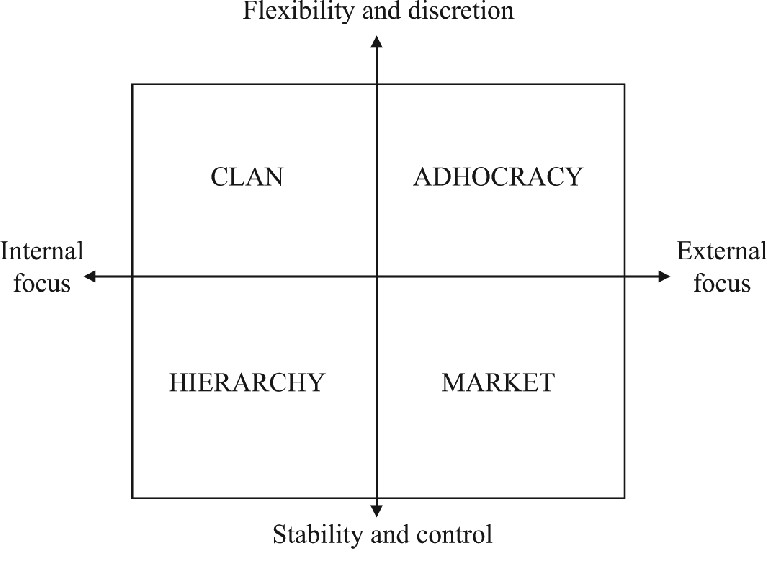
\includegraphics[width=0.5\textwidth]{cvf}
\caption{Modelo de Cameron \& Quinn}
\end{figure}

Estas dimensões definem uma dicotomia entre duas características de uma organização. Assim, a dimensão da flexibilidade/estabilidade impõe uma divisão entre organizações mais flexíveis e adaptáveis e, em contrapartida, organizações mais estáveis e controladoras. A dimensão de foco define uma dicotomia entre um foco de uma organização em processos internos ou em processos externos \parencite{diagnosing}.

Com estas divisões feitas, podemos definir os 4 tipos de culturas organizacionais:

\begin{itemize}
	\item \textit{Clan}
	\item \textit{Adhocracy}
	\item \textit{Hierarchy}
	\item \textit{Market}
\end{itemize}

\subsubsection{\textit{Clan}}

Esta cultura é definida por ter um foco interno e flexibilidade na manutenção da organização. Direciona-se para as pessoas afetas à organização. Esta tipologia é identificada, de forma geral, em organizações familiares.


\subsubsection{\textit{Adhocracy}}

Esta tipologia define uma cultura flexível e focada no mercado. Dá especial importância à inovação e empreendedorismo. Este tipo de organização é encontrado em mercados em rápido crescimento e com uma baixa aversão a risco.

\subsubsection{\textit{Hierarchy}}

Esta tipologia define uma cultura estável, controlada e com um foco interno. Enfatiza a eficiência e controlo dos processos organizacionais e a eliminação de erros. Este tipo de organização representa em grande parte organizações burocráticas com estruturas rígidas e bem-definidas.

\subsubsection{\textit{Market}}

Esta tipologia define uma cultura estável, controlado e com um foco no mercado. Assim, a organização está direcionada para a competição, em atingir objetivos. Esta tipologia adequa-se a empresas de marketing e vendas, por exemplo.

\subsection{Modelo de Hofstede}

No final do século XX, Geert Hofstede realizou um estudo em larga escala sobre as diferenças nos valores nacionais nas várias subsidiárias da empresa multinacional \acrfull{ibm}. Este estudo permitiu a Hofstede fazer comparações entre nações e realçar valores culturais que podem ser encontrados nos ambientes organizacionais. Hofstede posteriormente publicou um livro com os resultados desta pesquisa  \parencite{Hofstede_1981}.
 
Desse estudo resultou uma teoria chamada “A Teoria das Dimensões Culturais”. Esta permite examinar a forma como os valores culturais afetam o comportamento e as ações de pessoas de uma determinada cultura. A teoria divide-se em seis dimensões culturais: distância hierárquica, individualismo/coletivismo, aversão/incerteza, masculinidade/feminilidade, orientação em longo prazo e complacência/repressão.

\subsubsection{Distância hierárquica}

Aqui, o poder é distribuído de forma desigual, pois há uma necessidade de distinguir os superiores hierárquicos dos restantes. Estes últimos devem aceitar esta condição e esperar uma distribuição desigual do poder.

Neste conceito, a mudança acontece através de revoluções devido ao facto dos superiores hierárquicos terem privilégios.

\subsubsection{Individualismo vs Coletivismo}

O individualismo implica uma sociedade em que as decisões são tomadas de forma independente, em benefício próprio e com preocupações apontadas a si mesmo ou à família mais próxima.

Contrariamente, o coletivismo foca mais na relação dentro da sociedade do que nas tarefas individuais. Outro objetivo é  também manter a harmonia nos membros do grupo.

\subsubsection{Masculinidade vs Feminilidade}

Este fator tem como objetivo medir os graus dos valores associados ao sexo masculino e feminino.
Por um lado, sociedades onde a masculinidade prevalece, as pessoas são guiadas mais pelos resultados e ambição. Nestes casos, os conflitos são resolvidos de modo a vencerem os mais fortes.

Por outro lado, numa sociedade onde a feminilidade prevalece, a qualidade de vida é o foco principal juntamente com a harmonia interpessoal. Nestas situações, a sociedade tende a construir boas relações e sentir mais compaixão pelos menos afortunados.

\subsubsection{Evitamento da incerteza}

Este parâmetro representa a sensação de insegurança, desconforto e até medo que os colaboradores adotem perante o desconhecido, seja ele situações de risco, incertezas, imprevistos, etc. Este parâmetro varia de cultura para cultura e naquelas em que o índice de aversão à incerteza é mais elevado, as pessoas tendem a adotar um comportamento mais seguro de modo a evitar estas situações de risco e se sentirem melhor.

Os espaços culturais onde se identifica este comportamento e onde fugir à rotina significa maior ansiedade e stress são: Japão, Rússia, Grécia. Já em culturas onde o índice de aversão à incerteza é mais baixo, a sociedade adapta-se mais facilmente a situações de risco e incerteza sendo mais flexíveis dependendo das circunstâncias.

\subsubsection{\textit{Long-term vs short-term orientation}}

Em culturas onde o pensamento a longo prazo está constantemente presente, este é uma forma de incentivar a população a gerir melhor a sua economia, tendo a noção que os resultados poderão vir a aparecer lentamente, demonstrando assim serem pessoas pacientes, esforçadas e perseverantes. Com isto, estas apresentam estar dispostas a gerir os seus objetivos, sacrificando objetivos presentes por objetivos futuros mais recompensantes, ou seja frutos dos seus investimentos. 

Culturas que pensam a curto prazo são mais conservadoras e demonstram ser mais tradicionais. Defendem e incentivam o consumo, gastos e objetivos de curto prazo. Nestas sociedades, a “label” social imposta pelas pessoas envolventes é muito importante. Não demonstram grande importância com o que o futuro representa mas sim grande importância em viver o presente. Pode-se concluir que há uma grande pressão social relacionado com o estilo de vida de cada um e a imagem pública de cada um.

\subsubsection{Indulgência vs Restrição}

A predominância da indulgência numa população demonstra que a sua cultura valoriza o bem-estar e conexão humana. Procuram a satisfação de necessidades básicas e desejos. Não são pessoas materialistas, mas sim pessoas muito ligadas sentimentalmente entre si, o que leva a serem pessoas mais sociáveis, extrovertidas e amigáveis. Sendo assim estas pessoas mais facilmente conseguem apresentar empatia e perdoar o próximo.

Já em culturas onde predomina a restrição, a disciplina moral é muito relevante e importante. Existem normas sociais restritivas onde as pessoas sentem que os seus sentimentos são oprimidos prejudicando o seu bem-estar, tornando-as mais pessimistas, deprimidas e facilmente injustiçadas. São sociedades materialistas e que sobrevalorizam o seu status aos olhos da sociedade.